\section{Daten und Methoden}

\subsection{Methoden}
Die Daten wurden mit Hilfe von Python\cite{pythonPY}-Skripten untersucht. 
Zum Lesen und bearbeiten der Daten wurde das python-package pandas\cite{pandasPY} genutzt. Zur übersichtlichen Darstellung der Daten in Diagrammen wurden matplotlib\cite{matplotlibPY}, seaborn\cite{matplotlibPY} und ptitprince\cite{ptitprincePY} verwendet. 
Für die anschließende statistische Auswertung wurde außerdem
scipy\cite{scipyPY} genutzt.
Der Hergang der Analyse kann im Jupyter-Notebook \texttt{ab\_analysis.ipynb} nachvollzogen werden. 
Wenn in der Arbeit auf eine Codezelle \texttt{an\_<x>} hingewiesen wird, geht es um die entsprechende Zelle in diesem Notebook nach der Ausführung aller Zellen aufeinmal (\texttt{Run all}).
Funktionen wurden größtenteils ausgelagert und sind im \texttt{utils} Modul zu finden. 
Die Plots wurden im Jupyter-Notebook \texttt{ab\_plots.ipynb} erstellt.
Wenn in der Arbeit auf eine Codezelle \texttt{pl\_<x>} hingewiesen wird, geht es um die entsprechende Zelle in diesem Notebook nach der Ausführung aller Zellen aufeinmal (\texttt{Run all}).
Der gesamte Code befindet sich in der beiliegenden .zip Datei und kann jederzeit im GitHub Repository \href{https://github.com/Graunarmin/animal-bones}{animal-bones} eingesehen werden.

\subsection{Daten}
Alle untersuchten Daten stammen aus dem \href{https://archaeologydataservice.ac.uk/archives/view/abmap/}{Animal Bone Metrical Archive Project (ABMAP)}.
Der Datensatz des ABMAP enthält insgesamt knapp 61 000 Maße von über 24 700 Knochen aus mehr als 100 archäologischen Sammlungen.
Alle Knochen wurden in Südengland gefunden und wurden auf verschiedene Zeitintervalle zwischen 1000 v.Chr. und heute datiert. 
Hauptsächlich sind Knochen von Schafen, Ziegen und Rindern enthalten, aber es sind auch Daten von Schweinen, Pferden, Hunden, Hühnern, Gänsen und Katzen verfügbar. 
Da die Daten jedoch nur über eine \href{https://archaeologydataservice.ac.uk/archives/view/abmap/search.cfm}{Online-Datenbank} verfügbar sind und pro Anfrage maximal die ersten 10 000 Datenpunkte heruntergeladen werden können, wurde der Fokus dieser Arbeit auf eine Tierart gelegt, zu der es zwar weniger als 10 000 Einträge gibt, aber immer noch genug, um sie statistisch auswerten zu können. 
Die Spezies 'Horse' (Pferd) bot sich mit 3099 Einträge an.
Ein Problem bei der Untersuchung von Knochenmaßen ist immer, dass häufig weder Alter noch Rasse des Tieres exakt bestimmt werden können. Manche Knochentypen erlauben den Rückschluss eher als andere und bei manchen ist der Einfluss auf die Ergebnisse nur sehr gering, aber generell ist das Ausschließen von Jungtierknochen oft nicht möglich\cite{Driesch1976}.

\subsubsection{Erfasste Merkmale}
Der Datensatz ist multivariat, d.h. für jeden Knochen wurden mehrere Merkmale erfasst:
Jeder Datenpunkt ist ein Maß (\texttt{MEASURE}) in $mm$ einer bestimmten Messart (\texttt{MEASTYPE}) und wurde einem Knochen zugeordnet, wobei ein Knochen mehrere Maße haben kann. 
Jeder Knochen hat eine eindeutige ID (\texttt{BONEID}) und wurde einer Spezies zugeordnet (\texttt{SPECIES}). Außerdem wird angegeben, um welchen Knochentyp es sich jeweils handelt (\texttt{ELEMENT}) und von welcher Körperseite er stammt (\texttt{SIDE}).
Jeder Eintrag wurde absoult datiert (\texttt{RANGE}) und einer Periode der Urgeschichte zugeordnet (\texttt{PERIOD}) . 
Zusätzlich wurde jeweils der Fundort verzeichnet (\texttt{SITECODE}, \texttt{SITE}, \texttt{COUNTY}) und woher die ursprünglichen Daten stammen (\texttt{REFERENCE})
Zum Datenmanagement sind noch einige Metadaten verfügbar.

\subsection{Knochentypen}
Die 1038 Funde umfassen 14 verschiedene Knochentypen, welche in  \autoref{fig:horse_skeleton} \cite{WikiSkeletalHorse} übersichtlich dargestellt sind.
Da unterschiedliche Knochen unterschiedlich groß sind, ist ein Vergleich zwischen verschiedenen Knochentypen nicht sinnvoll. 
Stattdessen müssen die Daten nach den verschiedenen Knochentypen (Attribut \texttt{ELEMENT}) gruppiert und dann innerhalb dieser Gruppen untersucht werden.
Die Aufteilung in Gruppen nach Knochentyp geschieht in \texttt{an\_2}. 

\begin{figure}[H]
    \centering
    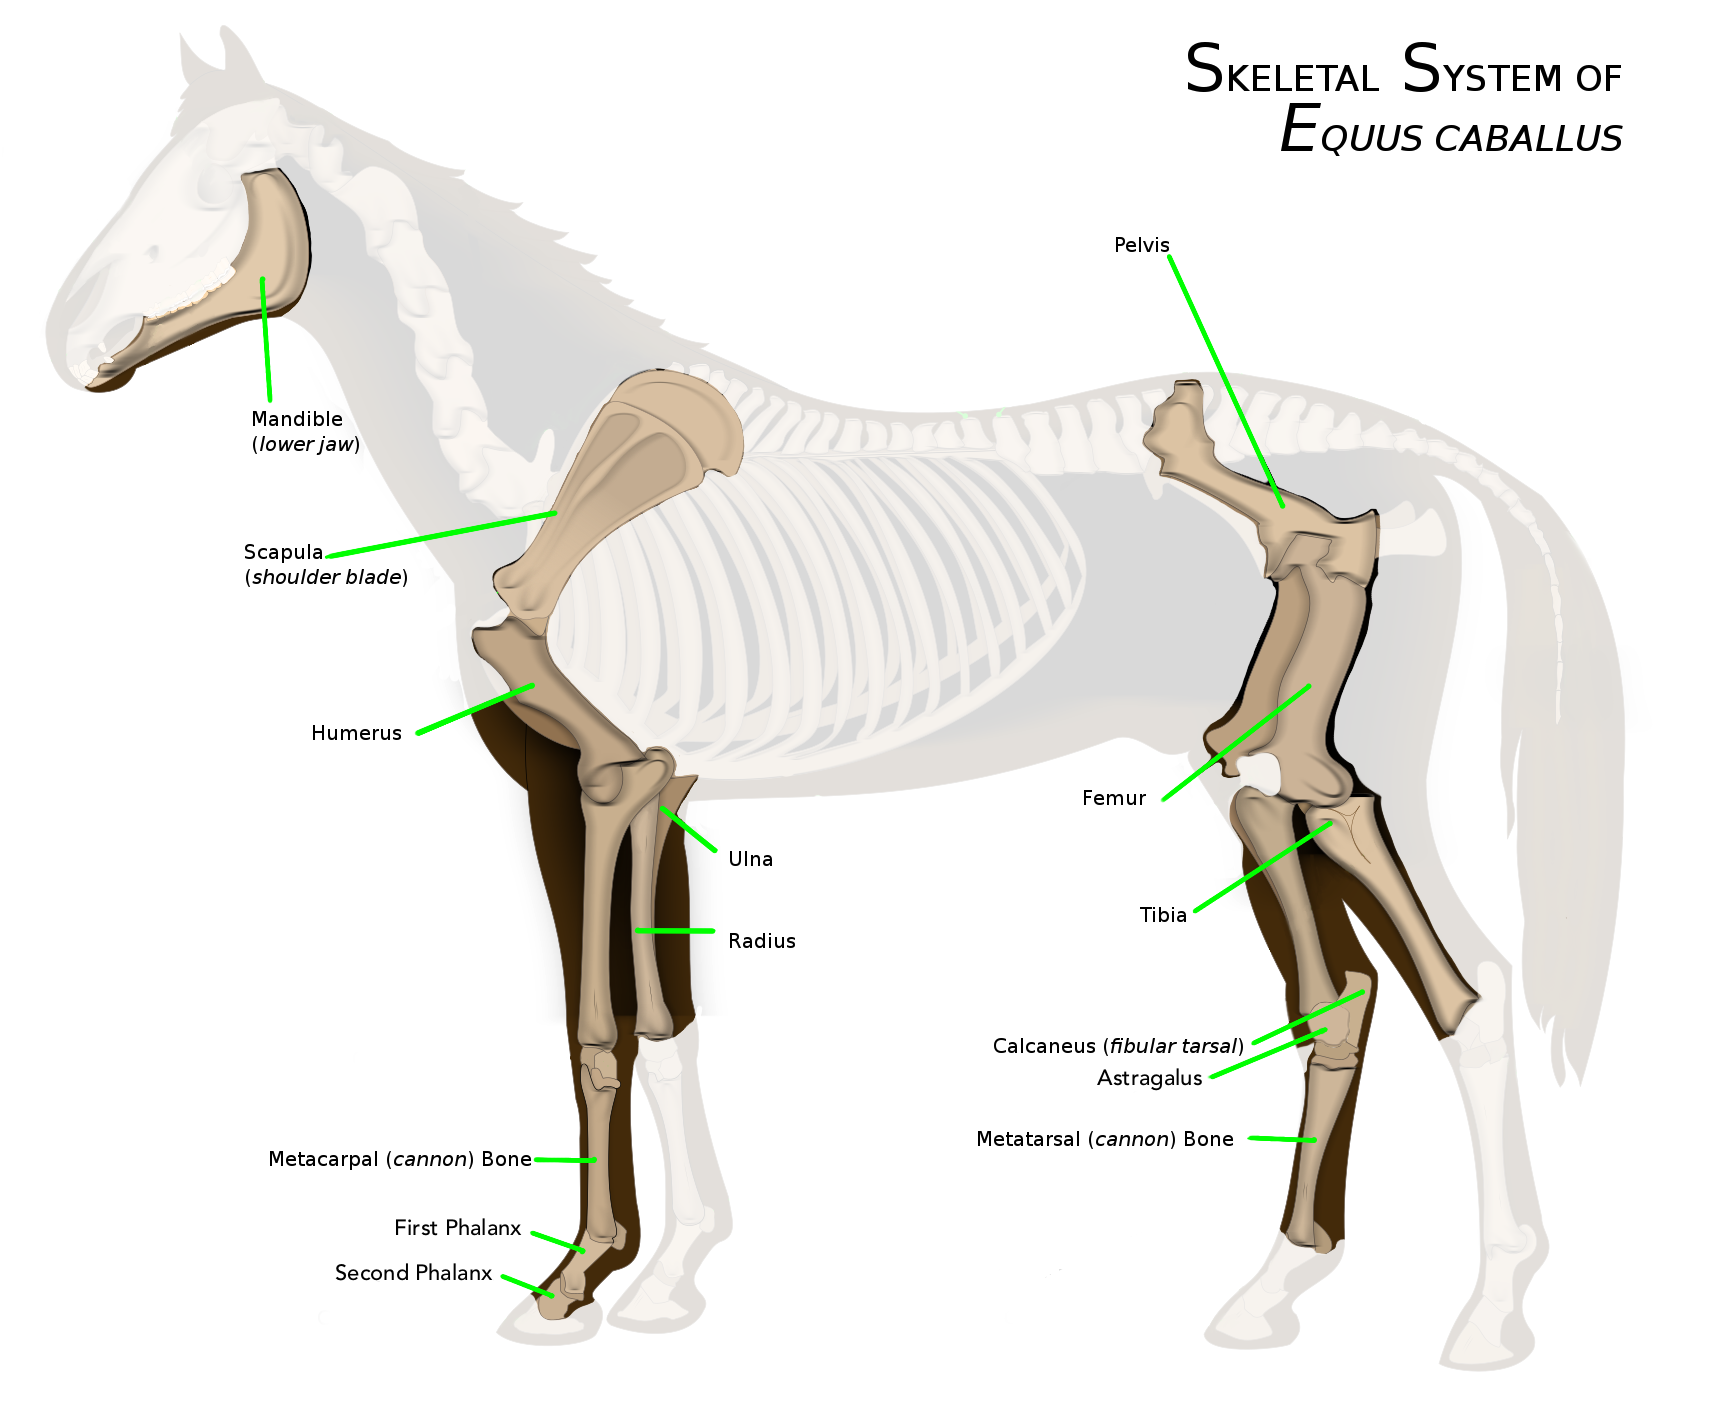
\includegraphics[height=10cm]{docs/latex/attachments/ab-project_Horse-anatomy.png}
    \caption{Die im Datensatz vorhandenen Knochen sind beschriftet und farblich hervorgehoben}
    \label{fig:horse_skeleton}
\end{figure}

\autoref{fig:barchart} zeigt jeweils die Menge an Funden und Messungen pro Knochentyp.

\begin{figure}[H]
    \centering
    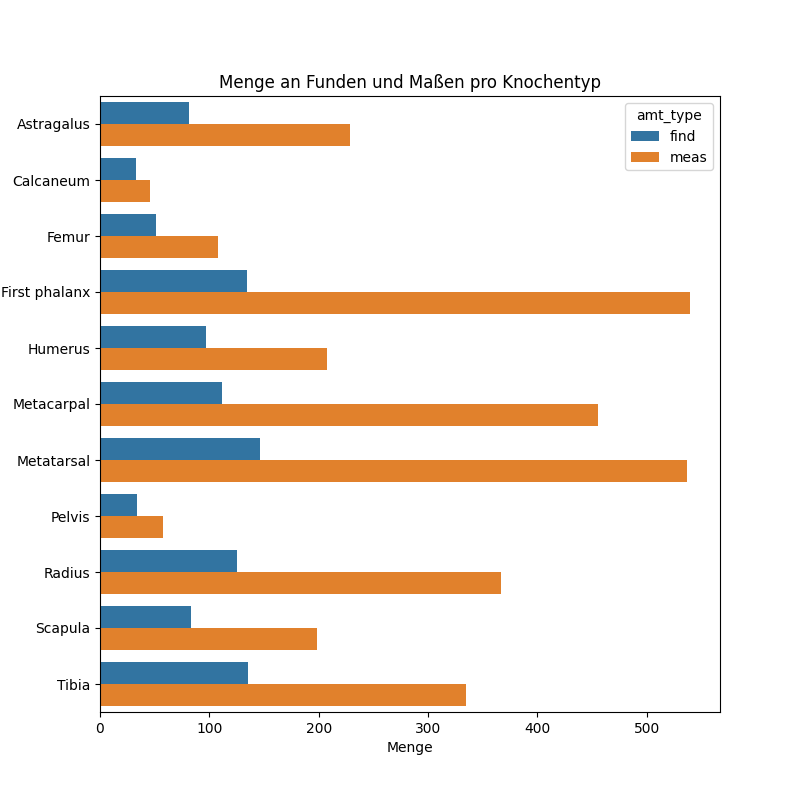
\includegraphics[height=10cm]{results/plots/amounts_barchart.png}
    \caption{Die Menge an Funden und Messungen pro Knochentyp}
    \label{fig:barchart}
\end{figure}


\subsection{Knochenmaße}

Jeder Knochen kann auf viele unterschiedliche Weisen vermessen werden, beispielsweise kann man den Umfang an einer bestimmten Stelle bestimmen, die Länge an der längsten Stelle oder die unterschiedlichen Breiten an den jeweiligen Enden oder in der Mitte. 
Diese verschiedenen »Dimensionen« wurden versucht, möglichst eindeutig zu definieren und damit zu standardisieren, doch \textit{»There will always be discrepancies from one research worker to the next which woll influence the final results.«} \cite{Driesch1976}
Im Datensatz wurden die unterschiedlichen Mess-Dimensionen durch das Attribut \texttt{MEASTYPE} gekennzeichnet, die verwendeten Codes beziehen sich größtenteils auf die Arbeit von \cite{Driesch1976}.
Wichtig ist an dieser Stelle vor allem zu beachten, dass auch die Maße für einen Vergleich nicht alle in einen Topf geworfen werden dürfen: Vermischt man Längenmaße mit Breite oder Umfang, verfälscht das das Ergebnis enorm.
Der Versuch, wenigstens unterschiedliche Dimensionen der gleichen Obergruppe (Länge, Breite, Umfang, Höhe) zusammenzufassen, wurde in \texttt{an\_9} und \texttt{an\_10} unternommen, doch aufgrund der Vielzahl und Komplexität der unterschiedlichen Messarten (und aufgrund des nicht vorhandenen Vorwissens der Autorin über Knochen, deren Bezeichnungen und Eigenarten) aufgegeben. 
Stattdessen wurden für jeden Knochentyp die vier Dimensionen mit den meisten Messwerten zur Weiterverarbeitung ausgewählt (s. \texttt{an\_11})

\subsection{Datierung}

Insgesamt liegen 101 unterschiedliche Zeitintervalle (\texttt{RANGE}) vor, welche insgesamt 21 Perioden zugeordnet wurden. Für die Betrachtung eines groben zeitlichen Trends sind 21 Perioden jedoch zu viele (und 101 Zeitintervalle erst recht). 
In \texttt{an\_6} bis \texttt{an\_8} wurden die Perioden und Ranges näher betrachtet mit der Absicht, die Einteilung zu vergröbern. Hierbei wurde jedoch ein Problem offensichtlich: die Funde überlappen sich teilweise in ihrer Datierung, sodass keine klaren Grenzen gezogen werden können, s. \autoref{fig:timeline}

\begin{figure}[H]
    \centering
    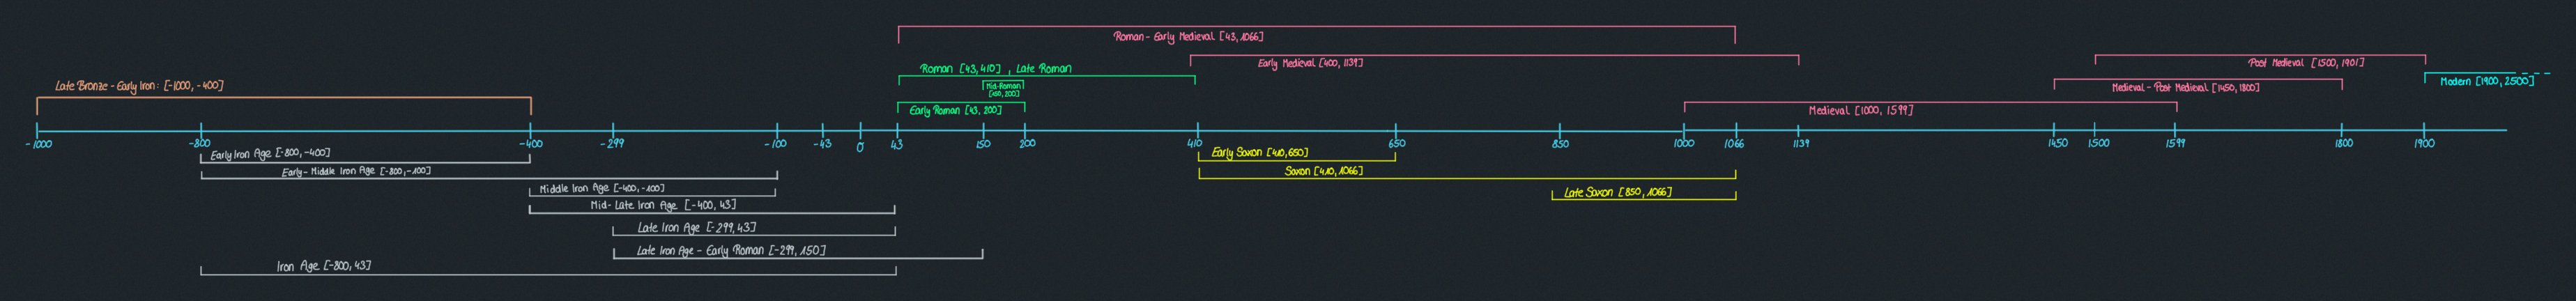
\includegraphics[width=\textwidth]{docs/latex/attachments/ab-project_timeline.png}
    \caption{Eine Skizze der im Datensatz definierten Perioden}
    \label{fig:timeline}
\end{figure}

Wenn ein Fund z.B. auf das Intervall zwischen -299 und 150 datiert wurde, ein anderer aber auf zwischen 43 und 200 kann man weder bei 150 noch bei 43 eine Grenze ziehen.
Daher werden die Funde wie in \autoref{fig:timeline_highlighted} grob in vier Zeitkategorien eingeteilt, um eine Betrachtung der Größenentwicklung über die Zeit zu ermöglichen. 
Die Überlappungen wurden in dieser Einteilung möglichst gering gehalten, lassen sich aber natürlich nicht ganz ausschließen.

\begin{figure}[H]
    \centering
    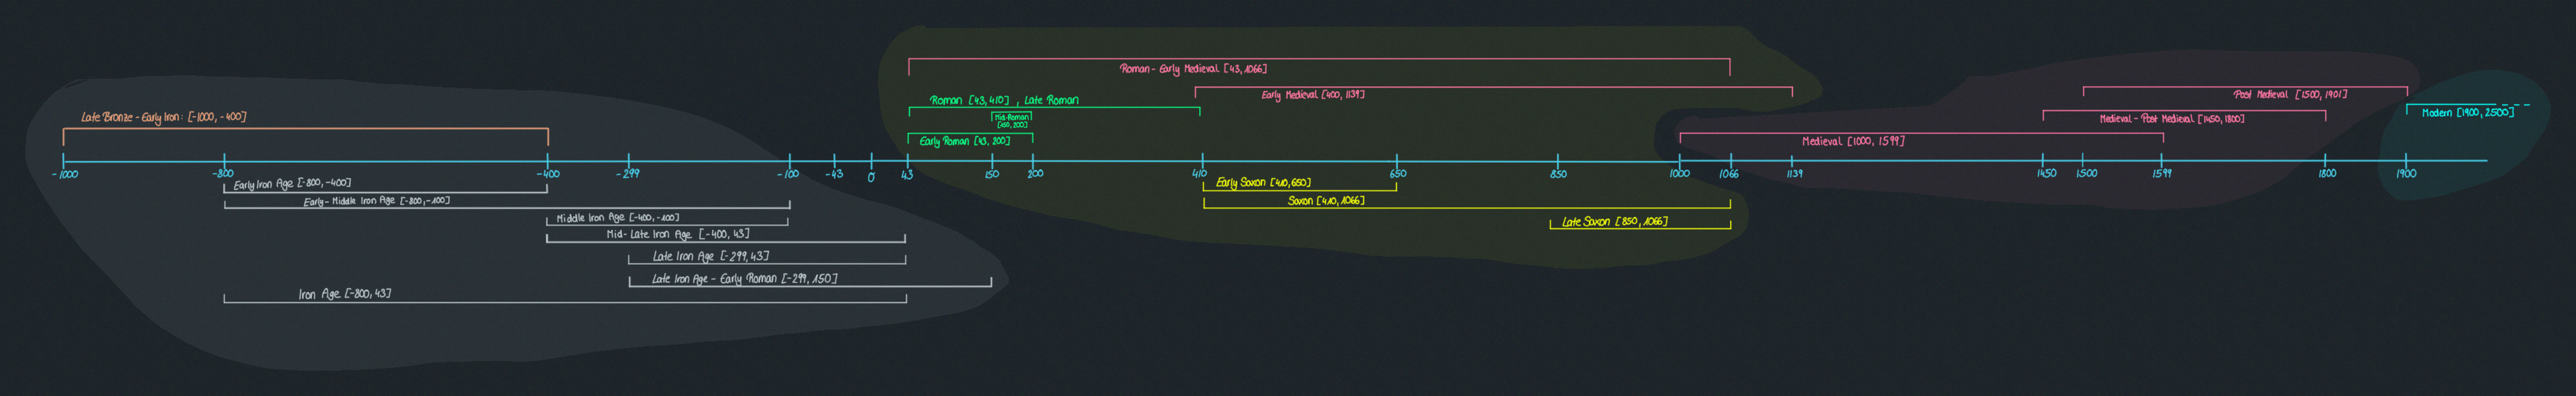
\includegraphics[width=\textwidth]{docs/latex/attachments/ab-project_timeline-highlighted.png}
    \caption{Die gewählten vier Gruppen wurden farblich hervorgehoben}
    \label{fig:timeline_highlighted}
\end{figure}

In \texttt{an\_7} wurde das \texttt{PERIOD}-Attribut der Funde entsprechend aktualisiert.

Figure 2.4 zeigt die Mengen der Funde und Messungen für alle Knochentypen pro Periode.
